\documentclass{article}[11pt]
\usepackage{graphicx}
\usepackage{tabularx}
\usepackage{natbib}


\usepackage{array}
\usepackage{amsmath}
%\usepackage[backend=bibtex]{biblatex}
\bibliographystyle{..//refs/styles/besjournals}
\setkeys{Gin}{width=0.8\textwidth}
%\setlength{\captionmargin}{30pt}
\setlength{\abovecaptionskip}{10pt}
\setlength{\belowcaptionskip}{10pt}
 \topmargin -1.5cm 
 \oddsidemargin -0.04cm 
 \evensidemargin -0.04cm 
 \textwidth 16.59cm
 \textheight 21.94cm 
 \parskip 7.2pt 
\renewcommand{\baselinestretch}{2}
\AtBeginEnvironment{thebibliography}{\linespread{1}\selectfont}
\parindent 0pt
\usepackage{lineno}
\linenumbers % for dissertation

\usepackage{xr-hyper}
\usepackage{hyperref}
\externaldocument{SUPPinvasive}
\externaldocument{JoE_rev_resp_parII}

\title{Contrasting responses to climate variability generate seasonal priority effects between native and invasive forest herbs} 
\author{D.M. Buonaiuto $^{1,2,3a}$, E.M. Wolkovich$^{2,3,4}$}

\date{}
\usepackage{Sweave}
\begin{document}
\input{invasive_wbbl_4_JoE-concordance}
\maketitle

\noindent \emph{Author affiliations:}\\
\noindent $^1$Department of Environmental Conservation, University of Massachusetts, Amherst, Massachusetts, USA. ORCID: 0000-0003-4022-2591\\
\noindent $^2$Arnold Arboretum of Harvard University, Boston, Massachusetts, USA.\\
$^3$Department of Organismic and Evolutionary Biology, Harvard University, Cambridge, Massachusetts, USA \\
$^4$Forest \& Conservation Sciences, Faculty of Forestry, University of British Columbia, Vancouver, British Columbia, Canada\\
$^a$Corresponding author: 617.823.0687; dbuonaiuto@umass.edu\\

\pagebreak
\section*{Abstract}
\begin{enumerate}
\item Invasive plants are often characterized by rapid germination and precocious phenology. Theory suggests that early germination may provide invaders with a competitive advantage over slower germinating natives, but the relative contribution of rapid germination vs. other intrinsic competitive traits\linelabel{tiny2} (e.g., rapid growth, high fecundity, broad environmental tolerance) to the success of invaders is poorly understood. Depending on the relationship between germination and competition, shifts in germination phenology due to climate change may increase the dominance of invaders or buffer communities against their impacts.

\item We investigated the link between temperature variation, germination phenology and competitive interactions with a sequence of controlled environment experiments. First, we evaluated the relationships between temperature variation and germination phenology for two herbaceous\linelabel{tiny1} species found in North American woodlands, the non-native \textit{Hesperis matronalis} and native \textit{Cryptotaenia canadensis}. We then leveraged temperature-response differences to manipulate the relative germination phenology of these taxa and quantified the effects of their phenological differences on competition.

\item Seeds of the invasive \textit{H. matronalis} germinated rapidly, reaching 50\% germination in under ten days in all treatment combinations. \textit{Cryptotaenia candensis} did not reach 50\% germination with less than seven weeks of cold stratification. However, with more than 10 weeks of cold stratification and low (20/10$^{\circ}$C) incubation temperatures, the germination phenology of \textit{C. canadensis} was well matched to that of \textit{H. matronalis}. When grown together, we found that precocious germination phenology doubled the competitive impact of \textit{H. matronalis} relative to its other intrinsic competitive traits. Phenological advantage of just two-three days relative to \textit{C. canadensis} was enough to secure competitive dominance at the seedling stage.

\item \textit{Synthesis.} This study revealed that the mechanistic link between the germination phenology and competitive success of an invasive plant can be strongly mediated by climate sensitivity differences between introduced and native species. Climate change will likely exacerbate these differences, especially in regions where warming reduces cold stratification. Our findings suggest that phenological diversity in native plant communities is an important property of invasion resistance. The relationship between environmental variation, germination dynamics and competition provides a path forward for for ecasting climate change impacts on seasonal community assembly, and highlights the need to incorporate phenological diversity in restorations.

\end{enumerate}


Keywords: competition, climate change, germination, invasion, phenology, priority effects, stratification

\pagebreak
\section*{Introduction}
 A central tenet of community assembly theory is that the order of arrival of species mediates inter-specific interactions and can dictate the trajectory of community structure \citep{Fukami2015}. These historical contingencies, known as priority effects, alter the structure and function of communities, driving communities to long-term alternate stable states \citep{Fukami2011}. Yet in many ecosystems, plant communities must re-assemble each year after a period of dormancy. In these communities, priority effects are the products of phenology, the timing of seasonal life cycle events, rather than the timing of the arrival of propagules, which occurs prior to the dormant season in many cases \citep{Rudolf:2019aa,Howe:1982aa,Baskin:1988aa}. 

Invasive plants are often characterized by rapid germination and precocious phenology under a wide variety of environmental conditions \citep{Gioria2018,Gioria:2017wo,Wolkovich:2011uh,Smith:2013uj}. By contrast, native plants tend to exhibit more constrained germination cues \citep{Marushia:2010ug,Wainwright:2013tv,Van-Clef:2001to}. In many temperate systems, seeds of native plants are characterized\linelabel{tiny3} with deep physiological dormancy, requiring prolonged exposure to specific environmental conditions, such as cold stratification (cool temperatures of 0-10$^{\circ}$ C), to break dormancy and stimulate germination \citep{Brink:2013wr,Cavieres:2017aa,Bradford:2007tj}. 

These differences in germination physiology can yield strong differences in the relative germination phenology of invasive and native plants, with invaders germinating well before their native competitors \citep{Gioria:2017wo}. This difference in relative germination timing among species, which we refer to as \textbf{phenological advantage}, can contribute significantly to the competitive abilities, and ultimately invasion success, of invasive plants. By allowing them to begin drawing down seasonal resources and modifying their environment before their native competitors emerge \citep{Kardol2013}, invaders gain a competitive advantage through a \textbf{seasonal priority effect} \citep{Wainwright_2011}.

Despite the growing interest in seasonal priority effects, it has been difficult to quantify their overall contribution to the competitive success of invaders. Germination is notoriously difficult to monitor in the field, and rapid phenology often co-varies with other competitive traits \citep{Dickson2012,Milbau:2003vt,HAO:2009vh}. Because of these difficulties, many experiments vary phenological advantage by sowing competing seeds at different time intervals \citep{Young:2017aa}. While these experiments have provided strong evidence that phenological advantage---on the order of just days to weeks---can yield substantial priority effects \citep{Weidlich:2020aa}, their experimental set-up is difficult to translate into natural communities in which priority effects are mediated by climate, and difficult to use for forecasting. Understanding the role that phenological advantage plays in mediating the dynamics of interspecific competition is critical for predicting and managing the structure and function of plant communities in the face of anthropogenic climate change. 

Due to interspecific differences in responses to environmental variation, altered environmental conditions are already shifting community-wide patterns of germination \citep{Walck2011}. If patterns of germination are indeed tightly linked to the competitive dynamics of communities, then phenological re-organization is likely to shift the strength of species' interactions, change patterns of invasion, and strongly influence biological filtering of plant communities. 

In this study, we\linelabel{prob1} performed a sequence of experiments in controlled environments to link climate variation, phenological advantage, and seasonal priority effects to the competitive interactions of two\linelabel{occur1} woodland herbaceous species (the invasive \textit{Hesperis matronalis} and native \textit{Cryptotaenia canadensis}) that frequently co-occur in the understory of temperate forest regions of North America. First, we performed a series of germination assays under varying temperature regimes to address the question: 
\begin{quote}How does phenological advantage between two species with contrasting responses to environmental cues shift due to variable climate conditions?\end{quote}
We then used competition trials under contrasting environmental conditions to indirectly manipulate the phenological advantage between these two taxa to address a second question: \begin{quote}To what extent do seasonal priority effects generated by varying patterns of phenological advantage influence the competitive dynamics of seedlings?\end{quote}

Pairwise\linelabel{cav1} studies in controlled environments like this one identify and isolate the mechanisms involved in interspecific competition, and serve an important foundation for understanding temporal dynamics of species interactions in real communities. While studies such as ours lack the complexity of wild plant communities, they serve as an important proof of concept for the potential role of seasonal priority effects in temperate forests, a system in which they have not been widely explored. Further, by linking climate variation, phenological advantage, and seasonal priority effects, our study has important implications for how anthropogenic climate change will alter phenological assembly and, in turn, plant community interactions in the\linelabel{prob2} decades to come.

\section*{Materials and Methods}

\subsection*{Species selection}
We selected focal\linelabel{crit1} species based on several criteria. First, we were interested in species that were herbaceous, biennial or perennial plants occurring in temperate forest understories of eastern North America. Because we were interested in the outcomes of plant competition, we selected species with substantial evidence that the species co-occur (and thus potentially compete) in nature. Finally, given our aim of understanding seasonal priority effects through phenological advantage, we selected species with sufficiently different responses to environmental\linelabel{crit2} variation.

\subsection*{Focal species}
Dames Rocket (\textit{Hesperis matronalis}) is a herbaceous biennial/perennial species in the Brasicaeceae family, originally from Eurasia, and introduced to North America in the 19th century \citep{Francis:2009wz}. It  can rapidly invade  meadows, forest edges and woodlands, forming thick stands and excluding native vegetation \citep{Francis:2009wz}. It is currently listed as a noxious or invasive weed in several states and provinces in the United States and Canada \citep{Susko:2008ut}. Honewort (\textit{Cryptotania canadensis}) is a herbaceous perennial in the Apiaceae family, native to forests and woodlands of eastern and central North America \citep{Hawkins:2007vb}. Observations of each species\linelabel{occ1} indicate that they co-occur widely in these regions (Fig. \ref{fig:map}, Tab. \ref{tab:occoverlap} and see Supporting Information: ``Co-occurrence of focal species\linelabel{occ2} in nature").  

While their habitat requirements may be similar, the two species display substantially different germination strategies, making them a suitable model for our study. \textit{Cryptotaenia canadensis} seeds are classified with deep physiological dormancy and require a substantial period of cold moist stratification to release dormancy and initiate germination \citep{Baskin:1988um}. While some reports suggest that cold stratification enhances germination in \textit{H. matronalis} at cool incubation temperatures, several studies have demonstrated that fresh and after-ripened (dry-stored) seeds of \textit{H. matronalis} are capable of rapid and complete germination at a wide range of temperatures \citep{Susko:2008ut}. These contrasting\linelabel{crit3} germination strategies suggest that variation in phenological advantage between these species is likely mediated by environmental variation; especially variation in exposure to cold stratification conditions\linelabel{crit4}.

\subsection*{Experiment I: Germination Assays}
To investigate the relationship between environmental variation and relative germination timing among species, we obtained seeds of \textit{C. canadensis} from Prairie Moon Nursery (Winona, MN) and seeds of \textit{H. matronalis} from American Meadows (Shelburne, VT). We performed germination assays in the growth facilities of the Arnold Arboretum in Boston, Massachusetts, USA (42.3074$^{\circ}$ N, 71.1208$^{\circ}$ W). We assigned seeds to a fully-crossed set of twenty experimental treatments; 10 levels of cold stratification duration (0,2,4,5,6,7,8,9,11,13 weeks at 4$^{\circ}$C) and two levels of incubation temperature (warm---25$^{\circ}$C:15$^{\circ}$C (day/night), cool---20$^{\circ}$C:10$^{\circ}$C (day/night)).

\noindent  Prior to applying experimental treatments we performed a ``float test" in which all seeds were placed in distilled water, and unfilled seeds (floating) were removed from the experiment \citep{Baskin2014}. We imbibed the remaining seeds in distilled water for 24 hours and then placed 20 seeds for each species/ treatment combination in petri dishes on moist pool-filter sand, with three replicates per treatment. For the cold stratification treatments, we wrapped petri dishes in aluminum foil to prevent light exposure and placed them in a growth chamber at 4$^{\circ}$C. After each stratification interval, we transferred the petri dishes to their assigned incubation chamber for 25 days, moistening the germination substrate as necessary to maintain maximum saturation of the medium without flooding the seeds. We checked for new germinates every two days, defining a seed as germinated when its radical was visible \citep{Baskin2014}. We assessed the viability of any seeds that did not germinate in the 25 day incubation period by performing\linelabel{crush} a ``crush test" in which we applied pressure to the intact seed to evaluate its condition \citep{Baskin2014}. We excluded any seeds deemed unviable from all subsequent analyses. Due to the staggering of our stratification treatments the experiment took place between 27 August - 12 December 2018.

\subsection*{Experiment II: Competition Trials}
\noindent To quantify the contribution of seasonal priority effects to interspecific competition dynamics we performed competition trials under controlled conditions in a research greenhouse at the Arnold Arboretum from October 2020 - February 2021. We planted seeds of \textit{C. canadensis} and \textit{H. matronalis} into 8.9 cm square pots in a standard potting mix\linelabel{pot1} of bark, sphagnum peat moss, perlite, dolomite Lime (Sungro Metro-Mix 852), employing a response surface design where we varied both the overall density of seeds and proportion of each species in each pot \citep{Inouye2001}. High\linelabel{densy1} and low density treatments consisted of 14 and 8 seeds respectively to reflect the range of seedbank densities that have been reported in temperate forests \citep{Leckie:2000tb,Bossuyt:2002un,Decocq:2004tq}. Proportion treatments were 100:0\%, 25:75\%, 50:50\%, 75:25\%, 0:100\% (\textit{C. canadensis}:\textit{H. matronalis}). Each density by proportion treatment was replicated six\linelabel{densy2} times.

\noindent We randomly assigned half of the pots to short (45 days) and long (72 days) cold stratification treatments in dark growth chambers at 4$^{\circ}$C. We staggered the start of the treatments, so that at the conclusion of cold stratification, all pots were transferred to a heated greenhouse maintained at 15-25$^{\circ}$C with 14 hours of supplemental light. Germination was observed daily from 24 December 2020 - 13 January 2021 and every two days from 15 January 2021 - 01 February 2021. The locations of each pot in the greenhouse were randomly reassigned every three days to minimize any blocking effects on germination or growth.

\noident After 35 days we added 1 tsp per gallon of water of Peter’s 20-10-20 liquid feed fertilizer to all pots. After 62 days, we harvested the above-ground biomass from all pots, dried it for 48 hours at 60$^{\circ}$C, and recorded the dry weight of each species/pot.

\subsection*{Statistical analysis}
\subsubsection*{Germination Assays}
To assess interspecific differences in the relationship between germination rate and temperature variability, we fit a Bayesian mixed-effect accelerated failure time model \citep[AFT,][]{ONOFRI:2010tl} using a Weibull distribution for the likelihood function. We included weeks of stratification and incubation temperature and their interaction with species as fixed effects. The model written below is modified from \citet{ONOFRI:2010tl}.

$t_{50} &= t_0 \phi$

where $t_{50}$ is time to 50\% germination and corresponds to the germination times of a reference seed lot ($t_0$) multiplied by an ``acceleration factor" ($\phi$). The acceleration factor is a product of the experimental treatments of our study through the equation:

$\phi=exp(\beta_{sp}X_{sp} &+\beta_{strat}X_{strat} &+ \beta_{inc}X_{inc} &+ \beta_{stratXspecies}X_{strat}*X_{sp} &+ \beta_{incXspecies}X_{inc}*X_{sp} )$

where $X_{sp}$, $X_{strat}$ and $X_{inc}$ are the species, stratification and incubation treatment levels in our experiment, and  $\beta_{sp}$, $\beta_{strat}$, $\beta_{inc}$, $\beta_{stratXspecies}$ and $\beta_{incXspecies}$ are the estimated effects on $\phi$  for adding an additional week or stratification or degree of incubation for each species respectively.  

The AFT modeling framework let us robustly compare germination timing ($t_{50}$,  time to 50\% germination) even among treatments with different final germination percentages by accounting for viable seeds that did not germinate during our incubation window \citep{Soltani:2015aa,ONOFRI:2010tl}. One drawback of this approach is that this class of models assumes that all viable seeds will eventually germinate, which we would not expect in nature. For this reason, we considered any estimated $t_{50}$ values greater than 40 days to indicate that seeds would not reach 50\% germination under those conditions.  

\subsubsection*{Competition trials}
\noindent We quantified phenological advantage between species by subtracting the mean germination time of \textit{H. matronalis} from that of \textit{C. canadensis} in each pot. This allowed us to evaluate the effect of phenological advantage with a regression design \citep{Cottingham:2005ud}, with advantage values ranging from -1.3 to 9.5 (\textit{C. candensis} mean germination time 1.3 days earlier to 9.5 days later than \textit{H. matronalis}).

For each pot, we calculated the relative growth rate difference (RGRD) among species using the equation below, modified from \citet{Connolly2005}.\\

RGRD &= $ ln(\frac{Y_{Cc}}{y_{Cc}}) &- ln(\frac{Y_{Hm}}{y_{Hm}}) $\\

where $Y_{Hm}$ and $Y_{Cc}$ are the final biomass of the species at the end of the experiment and $y_{Hm}$ and $y_{Cc}$ are the initial biomass of the seeds planted at the outset of the experiment. For this calculation we obtained estimates of seed mass for our focal species from the Kew Gardens Seed Information Database \citep{kew}.  

We then modeled the effect of seedling density of \textit{C. canadensis}, \textit{H. matronalis} and phenological advantage using on RGRD. The model is written below:\\

$RGRD_i &= N(\alpha + \beta_{Hm}n_{Hm} + \beta_{Cc}n_{Cc} + \beta_{pri}MGT, \sigma_{RGRD}^2$)\\

where  $\beta_{Hm}$ and $\beta_{Cc}$ are known as the species influence parameters---representing the intrinsic competitive ability of each species---or the estimated effect of increasing the seedling density of each species by one individual on the RGRD \citep{Connolly2005}. $n_{Hm}$ and $n_{Cc}$ are the number of germinated individuals of \textit{H. matronalis} and \textit{C. canadensis} respectively. The relationship between the species influence parameters and $n_{Hm}$ and $n_{Cc}$ indicate that these parameter estimates are dependent on both the number of seeds planted (i.e. the seed bank in each pot) and the fraction of those seeds that germinated. This formulation allows our model to partition the effects of interspecific differences in germination phenology from the effects of interspecific differences in germination fraction under each environmental treatment. $\beta_{pri}$ is the priority effect, or the effect of increasing the difference in mean germination time between  \textit{H.matronalis} and \texit{C. canadensis} by one day.  In this formulation, $\alpha$ is an un-interpretable intercept \citep{Connolly2005}.

\subsection*{Model Implementation}
\noindent We fit all models using the R package ``brms" \citep{Burkner2018}.  We ran the model on four chains with 4000 iterations and a 3000 iteration warm-up for a total of 4000 posterior draws for each parameter, using weakly informative priors. We validated model performance by obtaining $\hat{R}$ values between 1 and 1.01, high effective sample sizes and no divergent transitions. For all models we report the mean posterior estimate along with 90\% uncertainty intervals (I_{90}).

\section*{Results}
\subsection*{Germination advantage}
\textit{H. matronalis} reached 50\% germination in under ten days for all environmental treatments, always exceeding 75\% germination regardless of environmental conditions (Fig. \ref{fig:timecourse}, \ref{fig:aft}, Tab. \ref{tab:germcomps}). Increasing cold stratification duration and incubation temperature only marginally enhanced the germination rate of this species (Fig. \ref{fig:aft}). By contrast, increasing incubation temperature had a delaying effect on the germination rate of \textit{C. canadensis}, suggesting that the mean 20$^{\circ}$C temperature of our warm incubation treatment is supra-optimal for the species (Fig. \ref{fig:aft}). Without sufficient cold stratification ($<$7 weeks for cool incubation and $<$10 weeks for warm incubation temperatures), seeds of  \textit{C. canadensis} did not reach 50\% germination during the duration of our experiment (Fig. \ref{fig:timecourse}, \ref{fig:aft}, Tab. \ref{tab:germcomps}). However, under long durations of cold stratification, germination rates of \textit{C.canadensis} began to converge on those of \textit{H. matronialis}, and at levels of stratification $>$10 weeks and cool incubation, the germination rate and fraction of \textit{C.canadensis} was well matched to that of \textit{H. matronalis} (Fig. \ref{fig:timecourse}, \ref{fig:aft}, Tab. \ref{tab:germcomps}).

\subsection*{Germination priority effects}
In the absence of phenological advantage, the influence  of adding one seedling of \textit{H. matronalis} to a pot community was almost 4X less than adding one \textit{C. canadensis} seedling on the pot-level RGRD (represented by the species' influence parameters---\textit{H. matronalis} ($\beta_{Hm}$): 0.13, $I_{90}$: \textit{0.08, 0.17}, \textit{C. canadensis} ($\beta_{Cc}$): -0.41, $I_{90}$: \textit{-0.46, -0.35}). Each day increase in the phenological advantage of \textit{ H. matronalis} had approximately the same influence on shifting the community biomass composition towards \textit{H. matronalis} as adding an individual of that species to the community (seasonal priority effect ($\beta_{pri}$): 0.15, $I_{90}$: \textit{0.09, 0.20}, Fig. \ref{fig:RGRD}, Tab. \ref{tab:RGRD}).

\section*{Discussion}
\subsection*{Environmental drivers of seasonal priority effects} 
Our results identify a natural mechanism---species' differential sensitivity to temperature---that can generate seasonal priority effects, and thus reshape the competitive landscape between native and invasive species. In the absence of phenological advantage, the intrinsic competitive abilities of each species in our study suggest that the native species, \textit{C. canadensis}, is the stronger competitor (Fig. \ref{fig:RGRD}). 

However, the influence of one day of phenological advantage for \textit{H. matronalis} virtually doubled its influence on the final community composition, suggesting that seasonal priority effects play a major role in the competitive success of \textit{H. matronalis} (Fig. \ref{fig:RGRD}). Our results\linelabel{mov1} indicate that \textit{C. canadensis} can compete with the invasive \textit{H. matronalis} at high relative abundance levels and/or when phenological advantage is low, joining a growing body of experiments demonstrating that relative germination phenology can function as a seasonal priority effect, enhancing the performance of the earliest germinating species at the expense of later germinants \citep{Korner2008,Dickson2012,Ross1972}.

Our findings advance decades of work on seasonal priority effects by connecting them directly to environmental variation and extending them to forest systems. While research on the importance of seasonal priority effects has increased in recent years, the vast majority of studies have focused on dry grassland communities, and typically introduce priority effects artificially --- by staggered planting of competitors \citep{Young:2017aa,Weidlich:2020aa}. In contrast, our experiment employed a more ecologically realistic mechanism---generating variation in phenological advantage indirectly by leveraging interspecific differences in germination responses to cold stratification. Our results suggest that seasonal priority effects can strongly influence seedling competition even in environments where germination phenology is primarily under temperature control. The results of our pair-wise competition trial suggests that seasonal priority effects, manifested through rapid germination phenology and propagule pressure, are mechanistically related to the competitive dominance, and---ultimately---invasion success of \textit{H. matronalis}. 

Despite\linelabel{coax1} having diverging physiological responses to stratification, our study revealed that under a range of climate conditions, species with different dormancy types can express nearly identical germination phenology. This supports recent evidence that the relationship between contrasting dormancy types and coexistence is strongly influenced by long term climate variability rather than static, within-season\linelabel{coax2} temporal niche partitioning \citep{Shriver:2017ud,CHESSON:1993vx}.

\subsection*{Seasonal priority effects and anthropogenic climate change}
The implications of our study for the role of climate variability in mediating seasonal priority effects is two-fold. First, our results suggest that interannual climate variability should generate both among- and within- season variation in competition strength among species, potentially driving species coexistence via the storage effect \citep{Chesson:2003ve}. Second, the key role we observed of climate in generating germination advantage and therefore seasonal priority effects suggests that sustained alteration to historic patterns of climate variability, like those driven by anthropogenic climate change, are likely to alter the dynamics of competing seedlings. Changing patterns of phenological assembly have downstream effects on the structure and function of plant communities \citep{Yang:2010ta,Piao:2019wd}.

In our study, the phenological advantage of \textit{H. matronalis} was maximized under shorter stratification periods and warmer incubation temperatures. This suggests that the warming temperatures associated with anthropogenic climate change may increase the magnitude of seasonal priority effects, largely due to the delay of germination in more climate-sensitive native species like \textit{C. canadensis}. Yet,\linelabel{cold1} because cold stratification occurs at intermediate, cool temperatures, net warming may actually increase the amount of cold stratification in some areas in which sub-zero temperatures become less frequent with warming. In these regions, warming could benefit species that are better adapted to cooler germination conditions, as has been documented in some communities in the\linelabel{cold2} field \citep{KIMBALL:2010vg}.

Interestingly, the difference in phenological advantage among our focal species was much higher in our germination assays than in our competition trials even at comparable levels of stratification. There are likely several explanations for these differences. First, we used different metrics of germination speed, time to 50\% germination ($t_{50}$) and mean germination time in each experiment. While the metrics are related and often confused, there are important differences between them that make one or the other more appropriate for the two types of experiments we ran (see Supporting Information: ``Measures of germination speed"). Second, the incubation temperatures in our greenhouse competition trials were more variable than in our growth chamber germination assays. The lower germination fractions we observed in \textit{C. canadensis} under greenhouse conditions suggest that the temperature range was likely supra-optimal for this species, and the lower germination fraction increased the difference between $t_{50}$ estimates and mean germination time measurements. Finally, we  conducted germination assays and competition trials in different growth media (filter sand vs. potting soil), which have different moisture retention and light transmissible capacities. Germination media can affect germination rates \citep{Baskin2014}, which may further explain differences among our two experiments.

Despite these differences, in both experiments increasing cold stratification duration advanced the germination phenology of \textit{C. canadensis} and weakly that of \textit{H. matronalis}, resulting in weaker phenological advantage for \textit{H. matronalis} at longer stratification levels (Fig. \ref{fig:aft}, Fig.  \ref{fig:MGTsup}). This suggests that the relationships between cold stratification and germination phenology we observed were robust. 

Climate change may also increase the risk of precocious phenology \citep{Inouye:2000ud}. While in our experiment, there was no cost to germinating too early, in natural systems, selection usually limits early activity. Across environments, optimum germination phenology is likely driven by a trade-off between maximizing the length of the growing season and the risk of exposure to damaging environmental episodes when germinating too early \citep{Augspurger:2017vu}. For example, in dry grassland ecosystems, the precocious germination of invasives has a substantial cost if water availability is too low \citep{Wainwright_2011}. In temperate forest ecosystems, the primary risk of early phenology is damage from late season frost \citep{Kollas:2014vn} and climate change is also altering the timing and frequency of frost events \citep{Ma:2019uf}. Understanding how climate change will reshape this tradeoff between seasonal priority effects and frost risk is a critical next step for understanding plant community interactions in an era of global change. 

\section*{A research agenda for assessing the role of seasonal priority effects in plant communites of temperate forests}

Our experiments offer an important proof of concept, extending the potential relevance of seasonal priority effects in mediating plant interactions outside the annual desert and grassland communities, in which they have primarily been studied, to herbaceous forest communities where variability in phenological assembly is primarily controlled by temperature variation. Of course, experiments in controlled environments lack the complexity of real ecological systems; thus there are many steps necessary to link these findings to field conditions, and better evaluate the role of seasonal priority effects in temperate forests.

Factors like\linelabel{source1} local adaptation and trans-generational plasticity can influence the germination behavior of seeds \citep{Donohue:2010uy,Baughman:2019ty}. In our study, we obtained seeds of each species from different source populations. While many germination traits are conserved at the species level, intra-specific variation that we did not capture in our study design could moderate the patterns we observed in our experiments. Follow-up studies that collect seeds from co-occurring populations from a gradient of habitats, could at once account for and estimate variation at the population\linelabel{source2} level. 

Additionally\linelabel{multi1}, ground-layer plant communities of temperate forests are species rich \citep{Whigham:2004wy}, and understanding the the role of priority effects in a multi-species context is a major need. While our study focused on pair-wise differences, future studies could address this limitation by performing trials with more species, both in controlled environments and under field conditions, to capture the complexity of phenological assembly in multi-species plant communities that comprise of diverse functional types, germination niches and life-history traits like temperate\linelabel{multi2} forests.

Some studies suggest that seasonal priority effects many be transient, though several studies that used staggered planting methods at similar scales to the phenological advantage we observed in our trials saw the influence of these initial priority effects on community composition maintained several seasons later \citep{Vaughn:2015wp,Young:2017aa,Torrez:2017to}. While we found that seasonal priority effects impacted competition among seedlings, our experiment did not quantify the role of seasonal priority effects in influencing the long-term, among-year dynamics of these species.

In perennial communities, these long term dynamics are even more difficult to assess. Many perennial herbs, \textit{C. canadensis} included, rely heavily on vegetative reproduction \citep{Hawkins:2005ve}, and competition between ramets, and between ramets and seedlings, may also impact species interactions in the long-term. Understanding how phenological differences across life stages of long-lived perennial plants affects competition is an important need for predicting how communities may be impacted by interannual environmental variation and climate change.  

While more research is needed, our results are promising in the context of native plant establishment; whether colonizing new areas due to range shifts, recovering from novel disturbances or ecological restoration. Indeed, there has been a growing call to increase phenological diversity in restoration planning \citep{Hess:2019vn}. Studies have found that including early active species in plantings can suppress the abundance of invaders in both grassland \citep{Cleland:2013wo} and forest ecosystems \citep{Schuster:2020ww}. At the same time, restoration mixes tend to lack species which fill the early season phenological niche \citep{Havens:2016vo}. The results of our study suggest that minimizing the priority effect conferred to invasive species due to rapid germination and early phenology by including species with similar, early phenological traits could be a powerful tool for managing plant invasions and restoring native ecosystems in an era of global change.

\section*{Conclusion}
By leveraging the differential germination sensitivities to environmental cues of two competing species to manipulate phenological advantage between them, we were able to quantify the contribution of seasonal priority effects gained through rapid phenology on the competitive ability of the invasive species \textit{H. matronalis}. We found that priority effects were approximately as strong as the intrinsic competitive traits of \textit{H. matronalis} in influencing its competitive dominance over the native forest herb \textit{C. canadensis}, suggesting seasonal priority effects mechanistically increase the invasion success of \textit{H. matronalis}. Variation in germination phenology was strongly mediated by differences in how species respond to temperature cues, suggesting that sustained climate change will alter patterns of phenological advantage, potentially strengthening the seasonal priority effects of invaders as climate warms. Our findings highlight the important role of phenological diversity in the invasion resistance of native plant communities, implying that measures of phenological diversity should be incorporated into plant community assessments and ecological restoration. 

\section*{Author Contributions} 
D.M. Buonaiuto and E.M. Wolkovich conceived of this manuscript; D.M. Buonaiuto designed and executed the experiments, collected the data and performed the analyses; D.M. Buonaiuto led the writing of the manuscript. All authors contributed critically to drafts and gave final approval for submission.

\section*{Acknowledgements}
Special thanks to the two anonymous reviewers whose feedback helped shape this manuscript, and to K.J Woodruff, L. Toomey and the rest of the Arnold Arboretum research greenhouses staff for helping to manage the growth facilities as well as maintain and repeat these experiments throughout lab closures, quarantines and all other Covid19-related challenges.

\section*{Conflict of Interest}
The authors declare no conflict of interest.

\section*{Data Availability}
The data \citep{D-M-Buonaiuto:2023wj} from the germination assays and competition trials are available at KNB: The Knowledge Network for Biocomplexity (https://knb.ecoinformatics.org/view/doi:10.5063/F1ZG6QPW).

%\bibliography{..///refs/germination.bib}
\begin{thebibliography}{62}
\providecommand{\natexlab}[1]{#1}

\bibitem[{Augspurger \& Salk(2017)}]{Augspurger:2017vu}
Augspurger, C.K. \& Salk, C.F. (2017) Constraints of cold and shade on the
  phenology of spring ephemeral herb species. \emph{Journal of Ecology}
  \textbf{105}, 246--254.

\bibitem[{Baskin \& Baskin(2014)}]{Baskin2014}
Baskin, C. \& Baskin, J. (2014) \emph{Seeds: Ecology,Biogeography, and
  Evolution of Dormancy and Germination}. Elsevier Inc.

\bibitem[{Baskin \& Baskin(1988{\natexlab{a}})}]{Baskin:1988aa}
Baskin, C.C. \& Baskin, J.M. (1988{\natexlab{a}}) Germination ecophysiology of
  herbaceous plant species in a temperate region. \emph{American Journal of
  Botany} \textbf{75}, 286--305.

\bibitem[{Baskin \& Baskin(1988{\natexlab{b}})}]{Baskin:1988um}
Baskin, J.M. \& Baskin, C.C. (1988{\natexlab{b}}) The ecological life cycle of
  cryptotaenia canadensis (l.) dc. (umbelliferae), a woodland herb with
  monocarpic ramets. \emph{The American Midland Naturalist} \textbf{119},
  165--173.

\bibitem[{Baughman \emph{et~al.}(2019)Baughman, Agneray, Forister, Kilkenny,
  Espeland, Fiegener, Horning, Johnson, Kaye, Ott, St.~Clair \&
  Leger}]{Baughman:2019ty}
Baughman, O.W., Agneray, A.C., Forister, M.L., Kilkenny, F.F., Espeland, E.K.,
  Fiegener, R., Horning, M.E., Johnson, R.C., Kaye, T.N., Ott, J., St.~Clair,
  J.B. \& Leger, E.A. (2019) Strong patterns of intraspecific variation and
  local adaptation in great basin plants revealed through a review of 75 years
  of experiments. \emph{Ecology and Evolution} \textbf{9}, 6259--6275.

\bibitem[{Bossuyt \emph{et~al.}(2002)Bossuyt, Heyn \& Hermy}]{Bossuyt:2002un}
Bossuyt, B., Heyn, M. \& Hermy, M. (2002) Seed bank and vegetation composition
  of forest stands of varying age in central belgium: consequences for
  regeneration of ancient forest vegetation. \emph{Plant Ecology} \textbf{162},
  33--48.

\bibitem[{Bradford \& Nonogaki(2007)}]{Bradford:2007tj}
Bradford, K.J.K.J.. \& Nonogaki, H. (2007) \emph{Seed development, dormancy,
  and germination}. Blackwell Pub., Oxford, OX, UK; Ames, Iowa, USA.

\bibitem[{Buonaiuto \& Wolkovich (2023)}]{D-M-Buonaiuto:2023wj}
Buonaiuto, D.M., \& Wolkovich, E.M. (2023) Germination phenology and seedling competition
  between two forest herb species of the eastern united states in controlled
  enironments. \emph{Knowledge Network for Biocomplexity.
  doi:10.5063/F137775K.} .

\bibitem[{B{\"u}rkner(2018)}]{Burkner2018}
B{\"u}rkner, P.C. (2018) Advanced bayesian multilevel modeling with the r
  package brms. \emph{R Journal} \textbf{10}, 395--411.

\bibitem[{Cavieres \& Sierra-Almeida(2017)}]{Cavieres:2017aa}
Cavieres, L. \& Sierra-Almeida, A. (2017) Assessing the importance of
  cold-stratification for seed germination in alpine plant species of the
  high-andes of central chile. \emph{Perspectives in Plant Ecology, Evolution
  and Systematics} \textbf{30}.

\bibitem[{Chesson(2003)}]{Chesson:2003ve}
Chesson, P. (2003) Quantifying and testing coexistence mechanisms arising from
  recruitment fluctuations. \emph{Theoretical Population Biology} \textbf{64},
  345--357.

\bibitem[{CHESSON \& HUNTLY(1993)}]{CHESSON:1993vx}
Chesson, P. \& Huntley, N. (1993) Temporal hierarchies of variation and the
  maintenance of diversity. \emph{Plant Species Biology} \textbf{8}, 195--206.

\bibitem[{Cleland \emph{et~al.}(2013)Cleland, Larios \&
  Suding}]{Cleland:2013wo}
Cleland, E.E., Larios, L. \& Suding, K.N. (2013) Strengthening invasion filters
  to reassemble native plant communities: Soil resources and phenological
  overlap. \emph{Restoration Ecology} \textbf{21}, 390--398.

\bibitem[{Connolly \& Wayne({2005})}]{Connolly2005}
Connolly, J. \& Wayne, P. ({2005}) {Assessing determinants of community biomass
  composition in two-species plant competition studies}. \emph{Oecologia}
  \textbf{{142}}, {450--457}.

\bibitem[{Cottingham \emph{et~al.}(2005)Cottingham, Lennon \&
  Brown}]{Cottingham:2005ud}
Cottingham, K.L., Lennon, J.T. \& Brown, B.L. (2005) Knowing when to draw the
  line: designing more informative ecological experiments. \emph{Frontiers in
  Ecology and the Environment} \textbf{3}, 145--152.


\bibitem[{Decocq \emph{et~al.}(2004)Decocq, Valentin, Toussaint, Hendoux,
  Saguez \& Bardat}]{Decocq:2004tq}
Decocq, G., Valentin, B., Toussaint, B., Hendoux, F., Saguez, R. \& Bardat, J.
  (2004) Soil seed bank composition and diversity in a managed temperate
  deciduous forest. \emph{Biodiversity \& Conservation} \textbf{13},
  2485--2509.

\bibitem[{Dickson \emph{et~al.}(2012)Dickson, Hopwood \& Wilsey}]{Dickson2012}
Dickson, T.L., Hopwood, J.L. \& Wilsey, B.J. (2012) Do priority effects benefit
  invasive plants more than native plants? an experiment with six grassland
  species. \emph{Biological Invasions} \textbf{14}, 2617--2624.

\bibitem[{Donohue \emph{et~al.}(2010)Donohue, Rubio~de Casas, Burghardt, Kovach
  \& Willis}]{Donohue:2010uy}
Donohue, K., Rubio~de Casas, R., Burghardt, L., Kovach, K. \& Willis, C.G.
  (2010) Germination, postgermination adaptation, and species ecological
  ranges. \emph{Annual Review of Ecology, Evolution, and Systematics}
  \textbf{41}, 293--319.

\bibitem[{Francis \emph{et~al.}(2009)Francis, Cavers \&
  Warwick}]{Francis:2009wz}
Francis, A., Cavers, P.B. \& Warwick, S.I. (2009) The biology of canadian
  weeds. 140. hesperis matronalis l. \emph{Canadian Journal of Plant Science}
  \textbf{89}, 191--206.

\bibitem[{Fukami(2015)}]{Fukami2015}
Fukami, T. (2015) Historical contingency in community assembly: Integrating
  niches, species pools, and priority effects. \emph{Annual Review of Ecology,
  Evolution, and Systematics} \textbf{46}, 1--23.

\bibitem[{Fukami \& Nakajima({2011})}]{Fukami2011}
Fukami, T. \& Nakajima, M. ({2011}) {Community assembly: alternative stable
  states or alternative transient states?} \emph{Ecology Letters}
  \textbf{{14}}, {973--984}.

\bibitem[{{GBIF.org}(2023)}]{gbif}
{GBIF.org} (2023) Gbif occurrence download.

\bibitem[{Gioria \& Py{\v s}ek(2017)}]{Gioria:2017wo}
Gioria, M. \& Py{\v s}ek, P. (2017) Early bird catches the worm: germination as
  a critical step in plant invasion. \emph{Biological Invasions} \textbf{19},
  1055--1080.

\bibitem[{Gioria \emph{et~al.}(2018)Gioria, Py{\v s}ek \& Osborne}]{Gioria2018}
Gioria, M., Py{\v s}ek, P. \& Osborne, B.A. (2018) Timing is everything: does
  early and late germination favor invasions by herbaceous alien plants?
  \emph{Journal of Plant Ecology} \textbf{11}, 4--16.

\bibitem[{Hao \emph{et~al.}(2009)Hao, Qiang, Liu \& Cao}]{HAO:2009vh}
Hao, J.H., Qiang, S., Liu, Q.Q. \& Cao, F. (2009) Reproductive traits
  associated with invasiveness in conyza sumatrensis. \emph{Journal of
  Systematics and Evolution} \textbf{47}, 245--254.

\bibitem[{Havens \& Vitt(2016)}]{Havens:2016vo}
Havens, K. \& Vitt, P. (2016) The importance of phenological diversity in seed
  mixes for pollinator restoration. \emph{Natural Areas Journal} \textbf{36},
  531--537.

\bibitem[{Hawkins \emph{et~al.}(2005)Hawkins, Baskin \&
  Baskin}]{Hawkins:2005ve}
Hawkins, T.S., Baskin, J.M. \& Baskin, C.C. (2005) Life cycles and biomass
  allocation in seed- and ramet-derived plants of cryptotaenia canadensis
  (apiaceae), a monocarpic species of eastern north america. \emph{Canadian
  Journal of Botany} \textbf{83}, 518--528.

\bibitem[{Hawkins \emph{et~al.}(2007)Hawkins, Baskin \&
  Baskin}]{Hawkins:2007vb}
Hawkins, T.S., Baskin, J.M. \& Baskin, C.C. (2007) Seed morphology, germination
  phenology, and capacity to form a seed bank in six herbaceous layer apiaceae
  species of the eastern deciduous forest. \emph{Castanea} \textbf{72}, 8--14.

\bibitem[{Hess \emph{et~al.}(2019)Hess, Mesl{\'e}ard \& Buisson}]{Hess:2019vn}
Hess, M.C.M., Mesl{\'e}ard, F. \& Buisson, E. (2019) Priority effects: Emerging
  principles for invasive plant species management. \emph{Ecological
  Engineering} \textbf{127}, 48--57.

\bibitem[{Howe \& Smallwood(1982)}]{Howe:1982aa}
Howe, H.F. \& Smallwood, J. (1982) Ecology of seed dispersal \textbf{13},
  201--228.

\bibitem[{Inouye({2001})}]{Inouye2001}
Inouye, B. ({2001}) {Response surface experimental designs for investigating
  interspecific competition}. \emph{Ecology} \textbf{{82}}, {2696--2706}.

\bibitem[{Inouye(2000)}]{Inouye:2000ud}
Inouye, D.W. (2000) The ecological and evolutionary significance of frost in
  the context of climate change. \emph{Ecology Letters} \textbf{3}, 457--463.

\bibitem[{Kardol \emph{et~al.}({2013})Kardol, Souza \& Classen}]{Kardol2013}
Kardol, P., Souza, L. \& Classen, A.T. ({2013}) {Resource availability mediates
  the importance of priority effects in plant community assembly and ecosystem
  function}. \emph{Oikos} \textbf{{122}}, {84--94}.

\bibitem[{Kew(2022)}]{kew}
Kew, R.B.G. (2022) Seed information database (sid). version 7.1.

\bibitem[{KIMBALL \emph{et~al.}(2010)Kimball, Angert, Huxman \&
  Venable}]{KIMBALL:2010vg}
Kimball, S., Angert, A.L., Huxman, T.E. \& Venable, D.L. (2010) Contemporary
  climate change in the sonoran desert favors cold-adapted species.
  \emph{Global Change Biology} \textbf{16}, 1555--1565.

\bibitem[{Koerner \emph{et~al.}({2008})Koerner, Stoecklin, Reuther-Thiebaud \&
  Pelaez-Riedl}]{Korner2008}
Koerner, C., Stoecklin, J., Reuther-Thiebaud, L. \& Pelaez-Riedl, S. ({2008})
  {Small differences in arrival time influence composition and productivity of
  plant communities}. \emph{New Phytologist} \textbf{{177}}, {698--705}.

\bibitem[{Kollas \emph{et~al.}(2014)Kollas, K{\"o}rner \&
  Randin}]{Kollas:2014vn}
Kollas, C., K{\"o}rner, C. \& Randin, C.F. (2014) Spring frost and growing
  season length co-control the cold range limits of broad-leaved trees.
  \emph{Journal of Biogeography} \textbf{41}, 773--783.

\bibitem[{Leckie \emph{et~al.}(2000)Leckie, Vellend, Bell, Waterway \&
  Lechowicz}]{Leckie:2000tb}
Leckie, S., Vellend, M., Bell, G., Waterway, M.J. \& Lechowicz, M.J. (2000) The
  seed bank in an old-growth, temperate deciduous forest. \emph{Canadian
  Journal of Botany} \textbf{78}, 181--192.

\bibitem[{Ma \emph{et~al.}(2019)Ma, Huang, H{\"a}nninen \&
  Berninger}]{Ma:2019uf}
Ma, Q., Huang, J.G., H{\"a}nninen, H. \& Berninger, F. (2019) Divergent trends
  in the risk of spring frost damage to trees in europe with recent warming.
  \emph{Global Change Biology} \textbf{25}, 351--360.

\bibitem[{Marushia \emph{et~al.}(2010)Marushia, Cadotte \&
  Holt}]{Marushia:2010ug}
Marushia, R.G., Cadotte, M.W. \& Holt, J.S. (2010) Phenology as a basis for
  management of exotic annual plants in desert invasions. \emph{Journal of
  Applied Ecology} \textbf{47}, 1290--1299.

\bibitem[{Milbau \emph{et~al.}(2003)Milbau, Nijs, Van~Peer, Reheul \&
  De~Cauwer}]{Milbau:2003vt}
Milbau, A., Nijs, I., Van~Peer, L., Reheul, D. \& De~Cauwer, B. (2003)
  Disentangling invasiveness and invasibility during invasion in synthesized
  grassland communities. \emph{New Phytologist} \textbf{159}, 657--667.

\bibitem[{Onofri \emph{et~al.}(2010)Onofri, Gresta \& Tei}]{ONOFRI:2010tl}
Onofri, A., Gresta, F. \& Tei, F. (2010) A new method for the analysis of
  germination and emergence data of weed species. \emph{Weed Research}
  \textbf{50}, 187--198.

\bibitem[{Piao \emph{et~al.}(2019)Piao, Liu, Chen, Janssens, Fu, Dai, Liu,
  Lian, Shen \& Zhu}]{Piao:2019wd}
Piao, S., Liu, Q., Chen, A., Janssens, I.A., Fu, Y., Dai, J., Liu, L., Lian,
  X., Shen, M. \& Zhu, X. (2019) Plant phenology and global climate change:
  Current progresses and challenges. \emph{Global Change Biology} \textbf{25},
  1922--1940.

\bibitem[{Ross \& Harper(1972)}]{Ross1972}
Ross, M.A. \& Harper, J.L. (1972) Occupation of biological space during
  seedling establishment \textbf{60}, 77--88.

\bibitem[{Rudolf(2019)}]{Rudolf:2019aa}
Rudolf, V.H.W. (2019) The role of seasonal timing and phenological shifts for
  species coexistence. \emph{Ecology Letters} \textbf{22}, 1324--1338.

\bibitem[{Schuster \emph{et~al.}(2020)Schuster, Wragg, Williams, Butler,
  Stefanski \& Reich}]{Schuster:2020ww}
Schuster, M.J., Wragg, P.D., Williams, L.J., Butler, E.E., Stefanski, A. \&
  Reich, P.B. (2020) Phenology matters: Extended spring and autumn canopy cover
  increases biotic resistance of forests to invasion by common buckthorn
  (rhamnus cathartica). \emph{Forest Ecology and Management} \textbf{464},
  118067.

\bibitem[{Shriver(2017)}]{Shriver:2017ud}
Shriver, R.K. (2017) Rainfall variability and fine-scale life history tradeoffs
  help drive niche partitioning in a desert annual plant community.
  \emph{Ecology Letters} \textbf{20}, 1231--1241.

\bibitem[{Smith(2013)}]{Smith:2013uj}
Smith, L.M. (2013) Extended leaf phenology in deciduous forest invaders:
  mechanisms of impact on native communities. \emph{Journal of Vegetation
  Science} \textbf{24}, 979--987.

\bibitem[{Soltani \emph{et~al.}(2015)Soltani, Ghaderi-Far, Baskin \&
  Baskin}]{Soltani:2015aa}
Soltani, E., Ghaderi-Far, F., Baskin, C.C. \& Baskin, J.M. (2015) Problems with
  using mean germination time to calculate rate of seed germination.
  \emph{Australian Journal of Botany} \textbf{63}, 631--635.

\bibitem[{Susko \& Hussein(2008)}]{Susko:2008ut}
Susko, D.J. \& Hussein, Y. (2008) Factors affecting germination and emergence
  of dame's rocket (hesperis matronalis). \emph{Weed Science} \textbf{56},
  389--393.

\bibitem[{ten Brink \emph{et~al.}(2013)ten Brink, Hendriksma \&
  Bruun}]{Brink:2013wr}
ten Brink, D.J., Hendriksma, H.P. \& Bruun, H.H. (2013) Habitat specialization
  through germination cueing: a comparative study of herbs from forests and
  open habitats. \emph{Annals of Botany} \textbf{111}, 283--292.

\bibitem[{Torrez \emph{et~al.}(2017)Torrez, Mergeay, Meester, Honnay, Helsen \&
  Standish}]{Torrez:2017to}
Torrez, V., Mergeay, J., Meester, L.D., Honnay, O., Helsen, K. \& Standish, R.
  (2017) Differential effects of dominant and subordinate plant species on the
  establishment success of target species in a grassland restoration
  experiment. \emph{Applied vegetation science} \textbf{20}, 363--375.

\bibitem[{Van~Clef \& Stiles(2001)}]{Van-Clef:2001to}
Van~Clef, M. \& Stiles, E.W. (2001) Seed longevity in three pairs of native and
  non-native congeners: Assessing invasive potential. \emph{Northeastern
  Naturalist} \textbf{8}, 301--310.

\bibitem[{Vaughn \& Young(2015)}]{Vaughn:2015wp}
Vaughn, K.J. \& Young, T.P. (2015) Short-term priority over exotic annuals
  increases the initial density and longer-term cover of native perennial
  grasses. \emph{Ecological Applications} \textbf{25}, 791--799.

\bibitem[{Wainwright \& Cleland(2013)}]{Wainwright:2013tv}
Wainwright, C.E. \& Cleland, E.E. (2013) Exotic species display greater
  germination plasticity and higher germination rates than native species
  across multiple cues. \emph{Biological Invasions} \textbf{15}, 2253--2264.

\bibitem[{Wainwright \emph{et~al.}(2011)Wainwright, Wolkovich \&
  Cleland}]{Wainwright_2011}
Wainwright, C.E., Wolkovich, E.M. \& Cleland, E.E. (2011) Seasonal priority
  effects: implications for invasion and restoration in a semi-arid system.
  \emph{Journal of Applied Ecology} \textbf{49}, 234--241.

\bibitem[{Walck \emph{et~al.}({2011})Walck, Hidayati, Dixon, Thompson \&
  Poschlod}]{Walck2011}
Walck, J.L., Hidayati, S.N., Dixon, K.W., Thompson, K. \& Poschlod, P. ({2011})
  {Climate change and plant regeneration from seed}. \emph{Global Change
  Biology} \textbf{{17}}, {2145--2161}.

\bibitem[{Weidlich \emph{et~al.}(2020)Weidlich, Nelson, Maron, Callaway, Delory
  \& Temperton}]{Weidlich:2020aa}
Weidlich, E.W.A., Nelson, C.R., Maron, J.L., Callaway, R.M., Delory, B.M. \&
  Temperton, V.M. (2020) Priority effects and ecological restoration.
  \emph{Restoration Ecology} \textbf{n/a}, e13317.

\bibitem[{Whigham(2004)}]{Whigham:2004wy}
Whigham, D.F. (2004) Ecology of woodland herbs in temperate deciduous forests.
  \emph{Annual Review of Ecology, Evolution, and Systematics} \textbf{35},
  583--621.

\bibitem[{Wolkovich \& Cleland(2011)}]{Wolkovich:2011uh}
Wolkovich, E.M. \& Cleland, E.E. (2011) The phenology of plant invasions: a
  community ecology perspective. \emph{Frontiers in Ecology and the
  Environment} \textbf{9}, 287--294.

\bibitem[{Yang \& Rudolf(2010)}]{Yang:2010ta}
Yang, L.H. \& Rudolf, V.H.W. (2010) Phenology, ontogeny and the effects of
  climate change on the timing of species interactions. \emph{Ecology Letters}
  \textbf{13}, 1--10.

\bibitem[{Young \emph{et~al.}(2017)Young, Stuble, Balachowski \&
  Werner}]{Young:2017aa}
Young, T.P., Stuble, K.L., Balachowski, J.A. \& Werner, C.M. (2017) Using
  priority effects to manipulate competitive relationships in restoration.
  \emph{Restoration Ecology} \textbf{25}, S114--S123.

\end{thebibliography}

\section*{Figures}


\begin{figure}[h!] 
    \centering
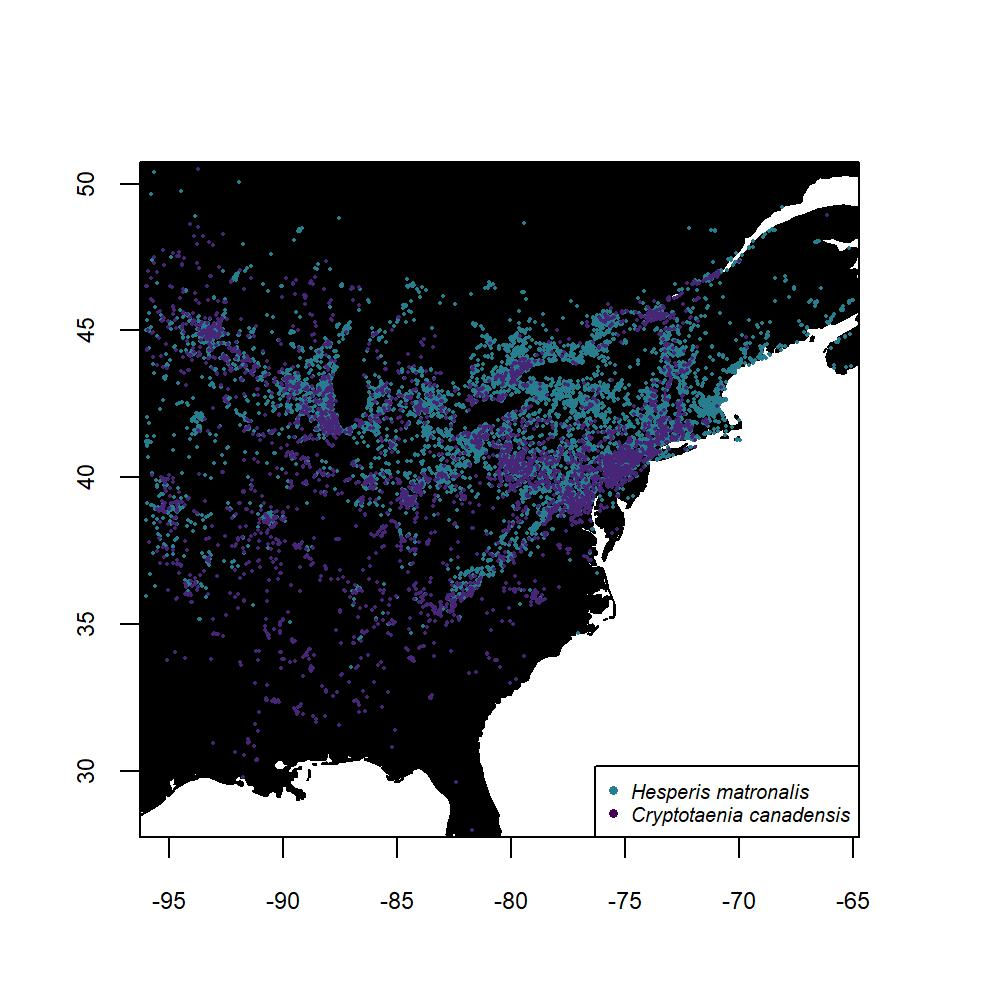
\includegraphics[width=.95\textwidth]{..//figure/cchhmmap4.jpeg}
\caption{Occurrence records of \textit{C. canadensis} and \textit{H. matronalis} in Eastern North America. Occurrence data were obtained from the Global Biodiversity Information Facility \citep[GBIF,][]{gbif}.} 
   \label{fig:map}
\end{figure}


\begin{figure}[h!]
    \centering
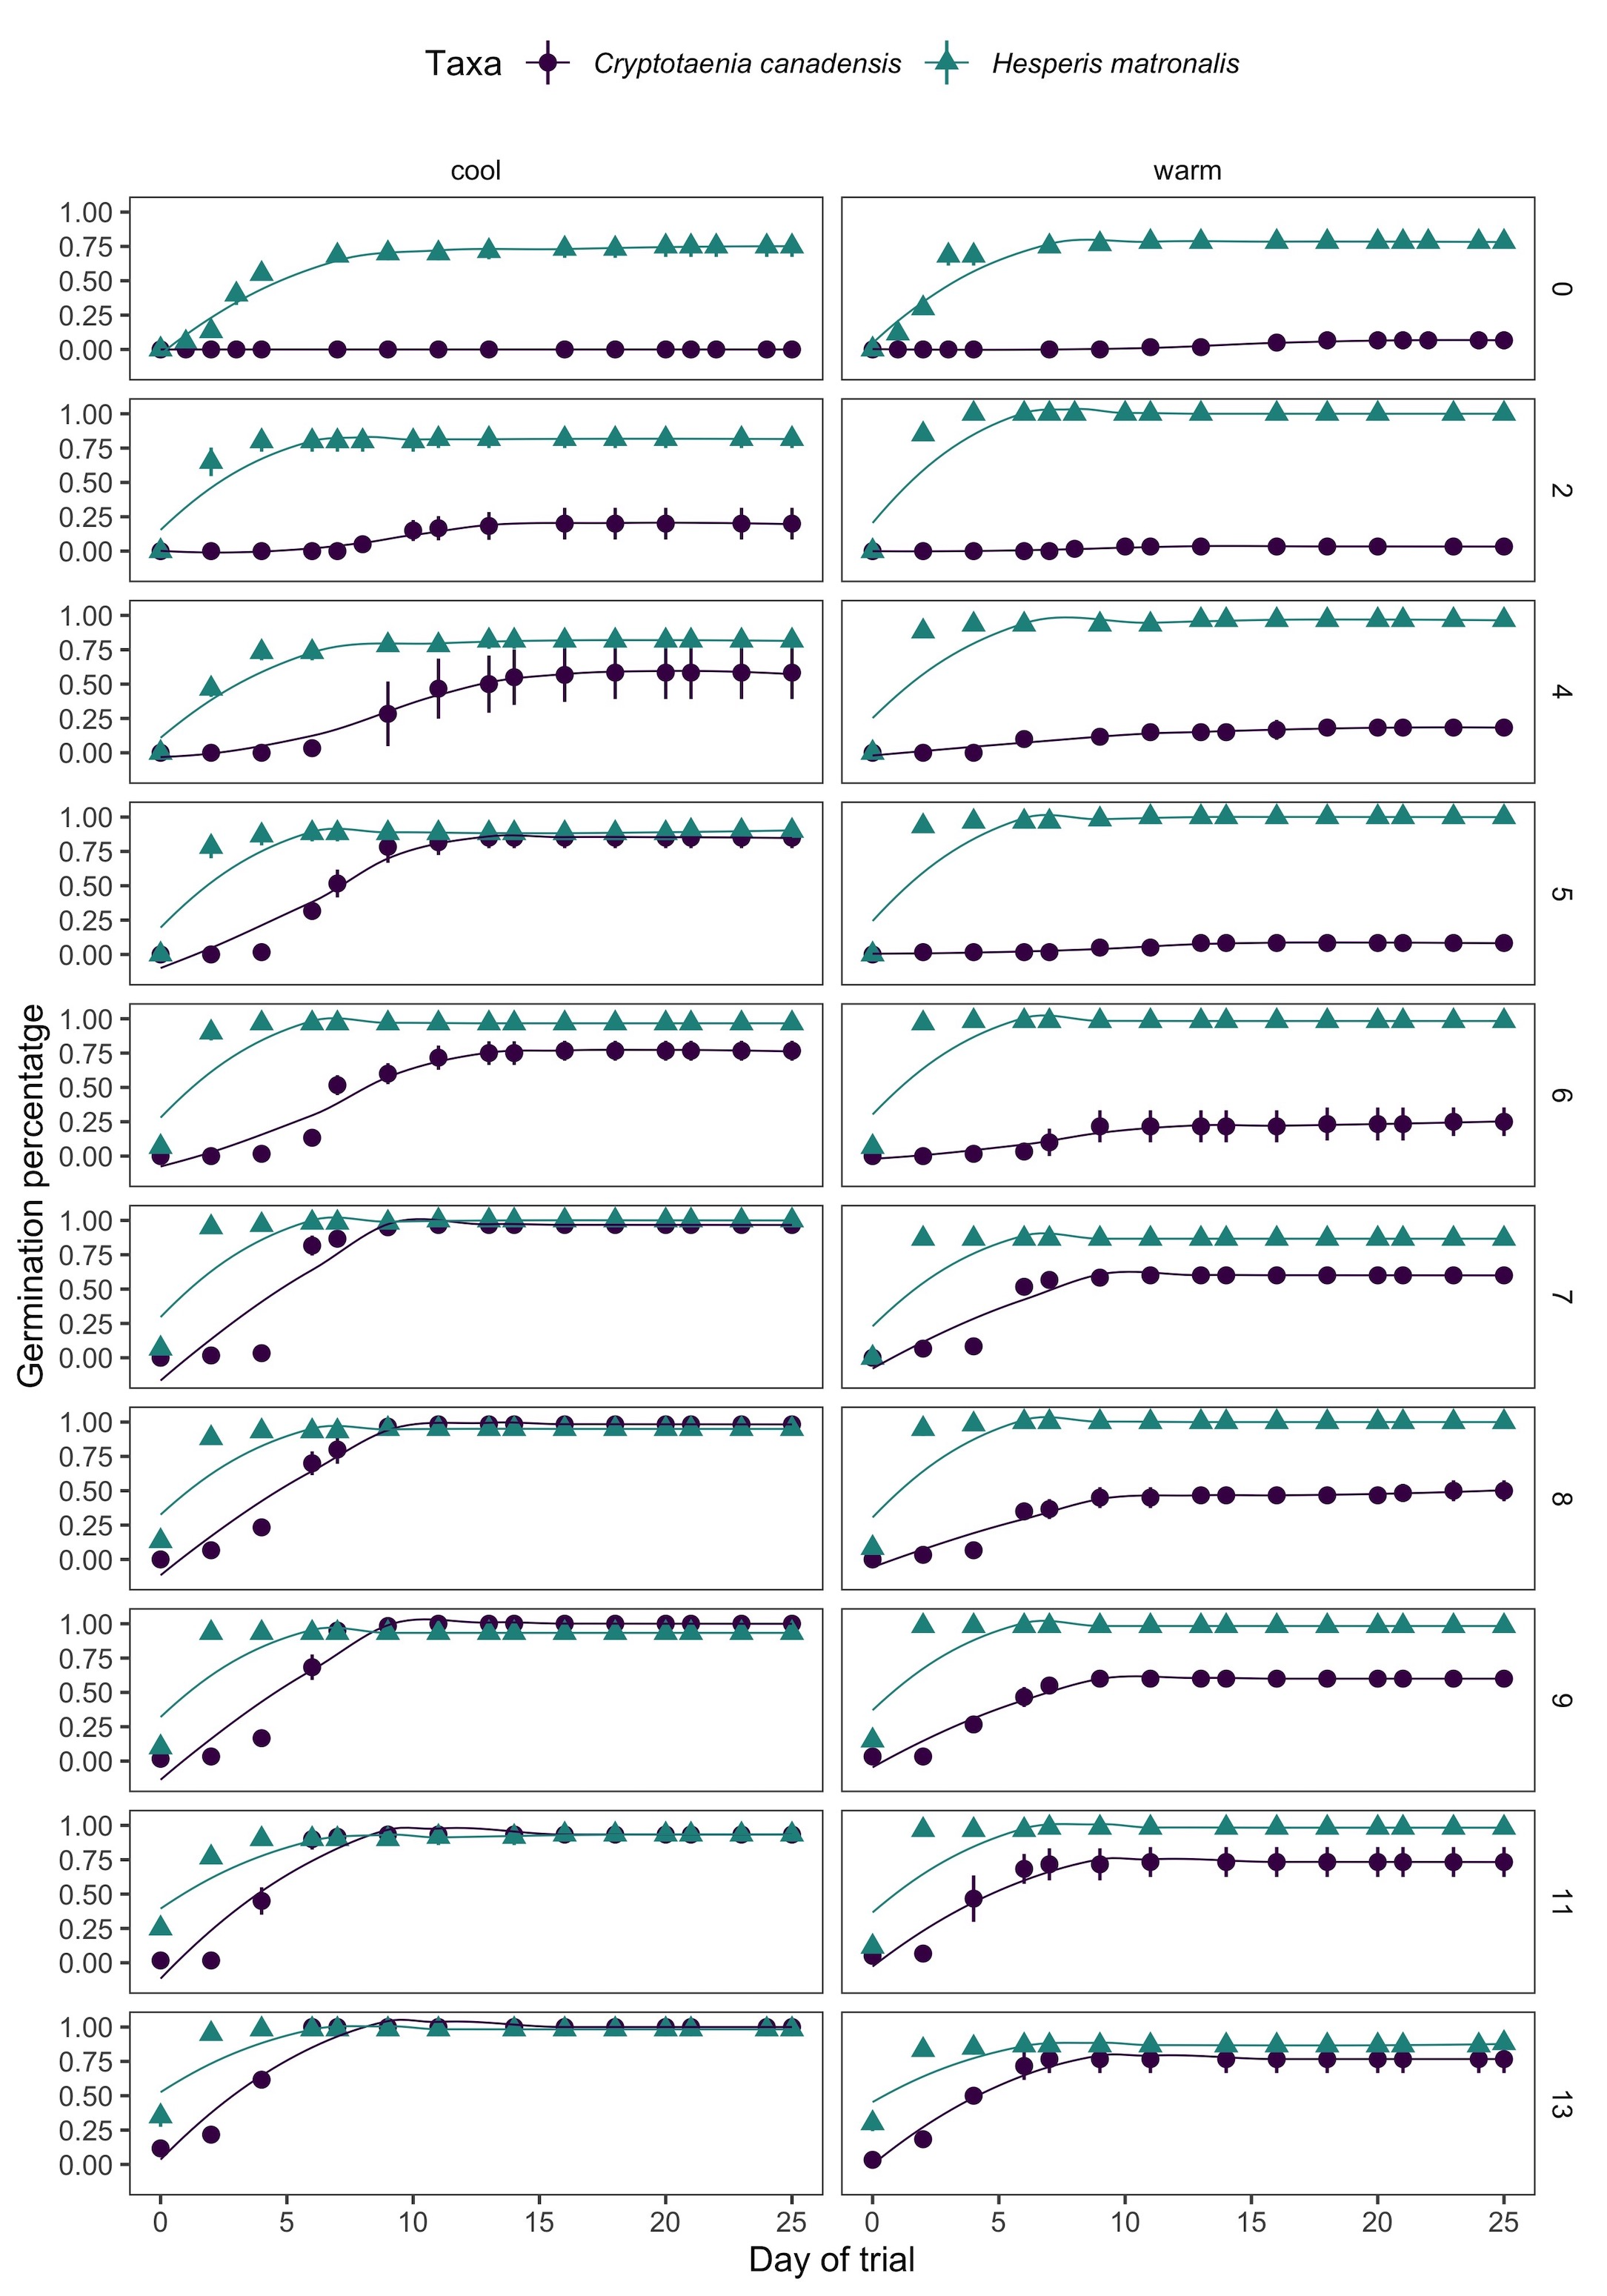
\includegraphics[width=.75\textwidth]{..//figure/crp_hesp2.jpeg}
\caption{Cumulative germination rates of \textit{H. matronalis} and \textit{C. canadensis} under cool (20/10$^{\circ}$ C day/night) and warm (25/15$^{\circ}$ C day/night) incubation temperatures for each stratification treatment (number of weeks at 4$^{\circ}$ C, right axis) in our germination assays. Points depict the mean cumulative germination at each observation time, and vertical bars depict the standard error across replicates. Lines represents a generalized trend for cumulative germination, fit with a loess function. See Fig. \ref{fig:aft} for model estimates from these data.}
   \label{fig:timecourse}
\end{figure}


\begin{figure}[h!]
    \centering
          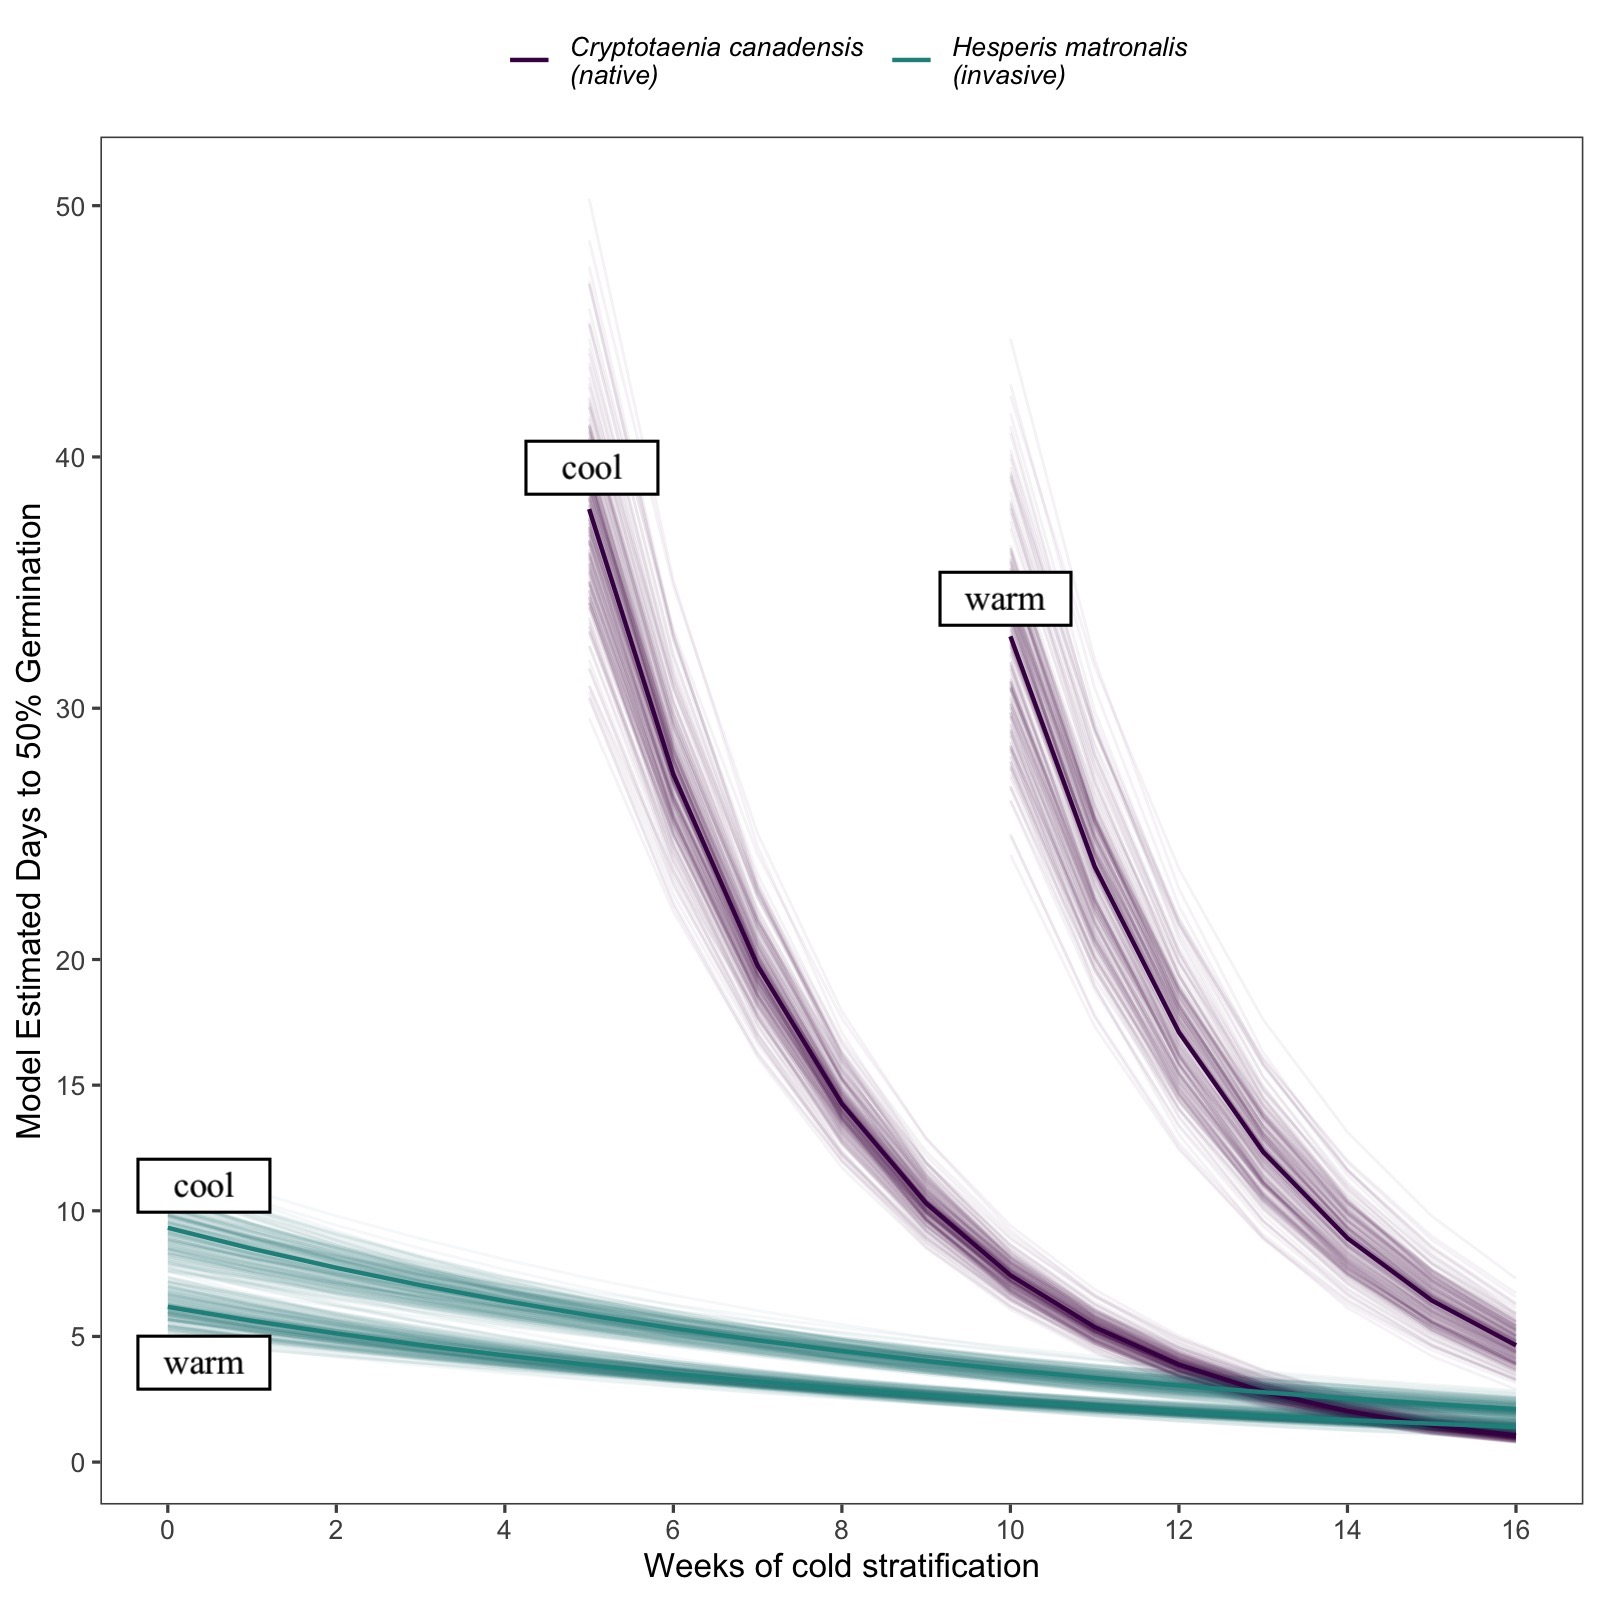
\includegraphics[width=\textwidth]{..//figure/AFTsivansive.jpeg}
   
\caption{The effects of weeks of cold stratification at 4$^{\circ}$ C on the time to 50\% germination of \textit {Cryptotaenia canadensis} and \textit{Hesperis matronalis} under warm (20/10$^{\circ}$ C day/night) and cool (25/15$^{\circ}$ C day/night) incubation conditions, estimated with an accelerated failure time model. We show here only stratification treatment levels which allowed both species to reach 50\% germination in less that 40 days. The solid lines depict the mean estimate, while lighter lines depict uncertainty.}
    \label{fig:aft}
\end{figure}


\begin{figure}[h!]
    \centering
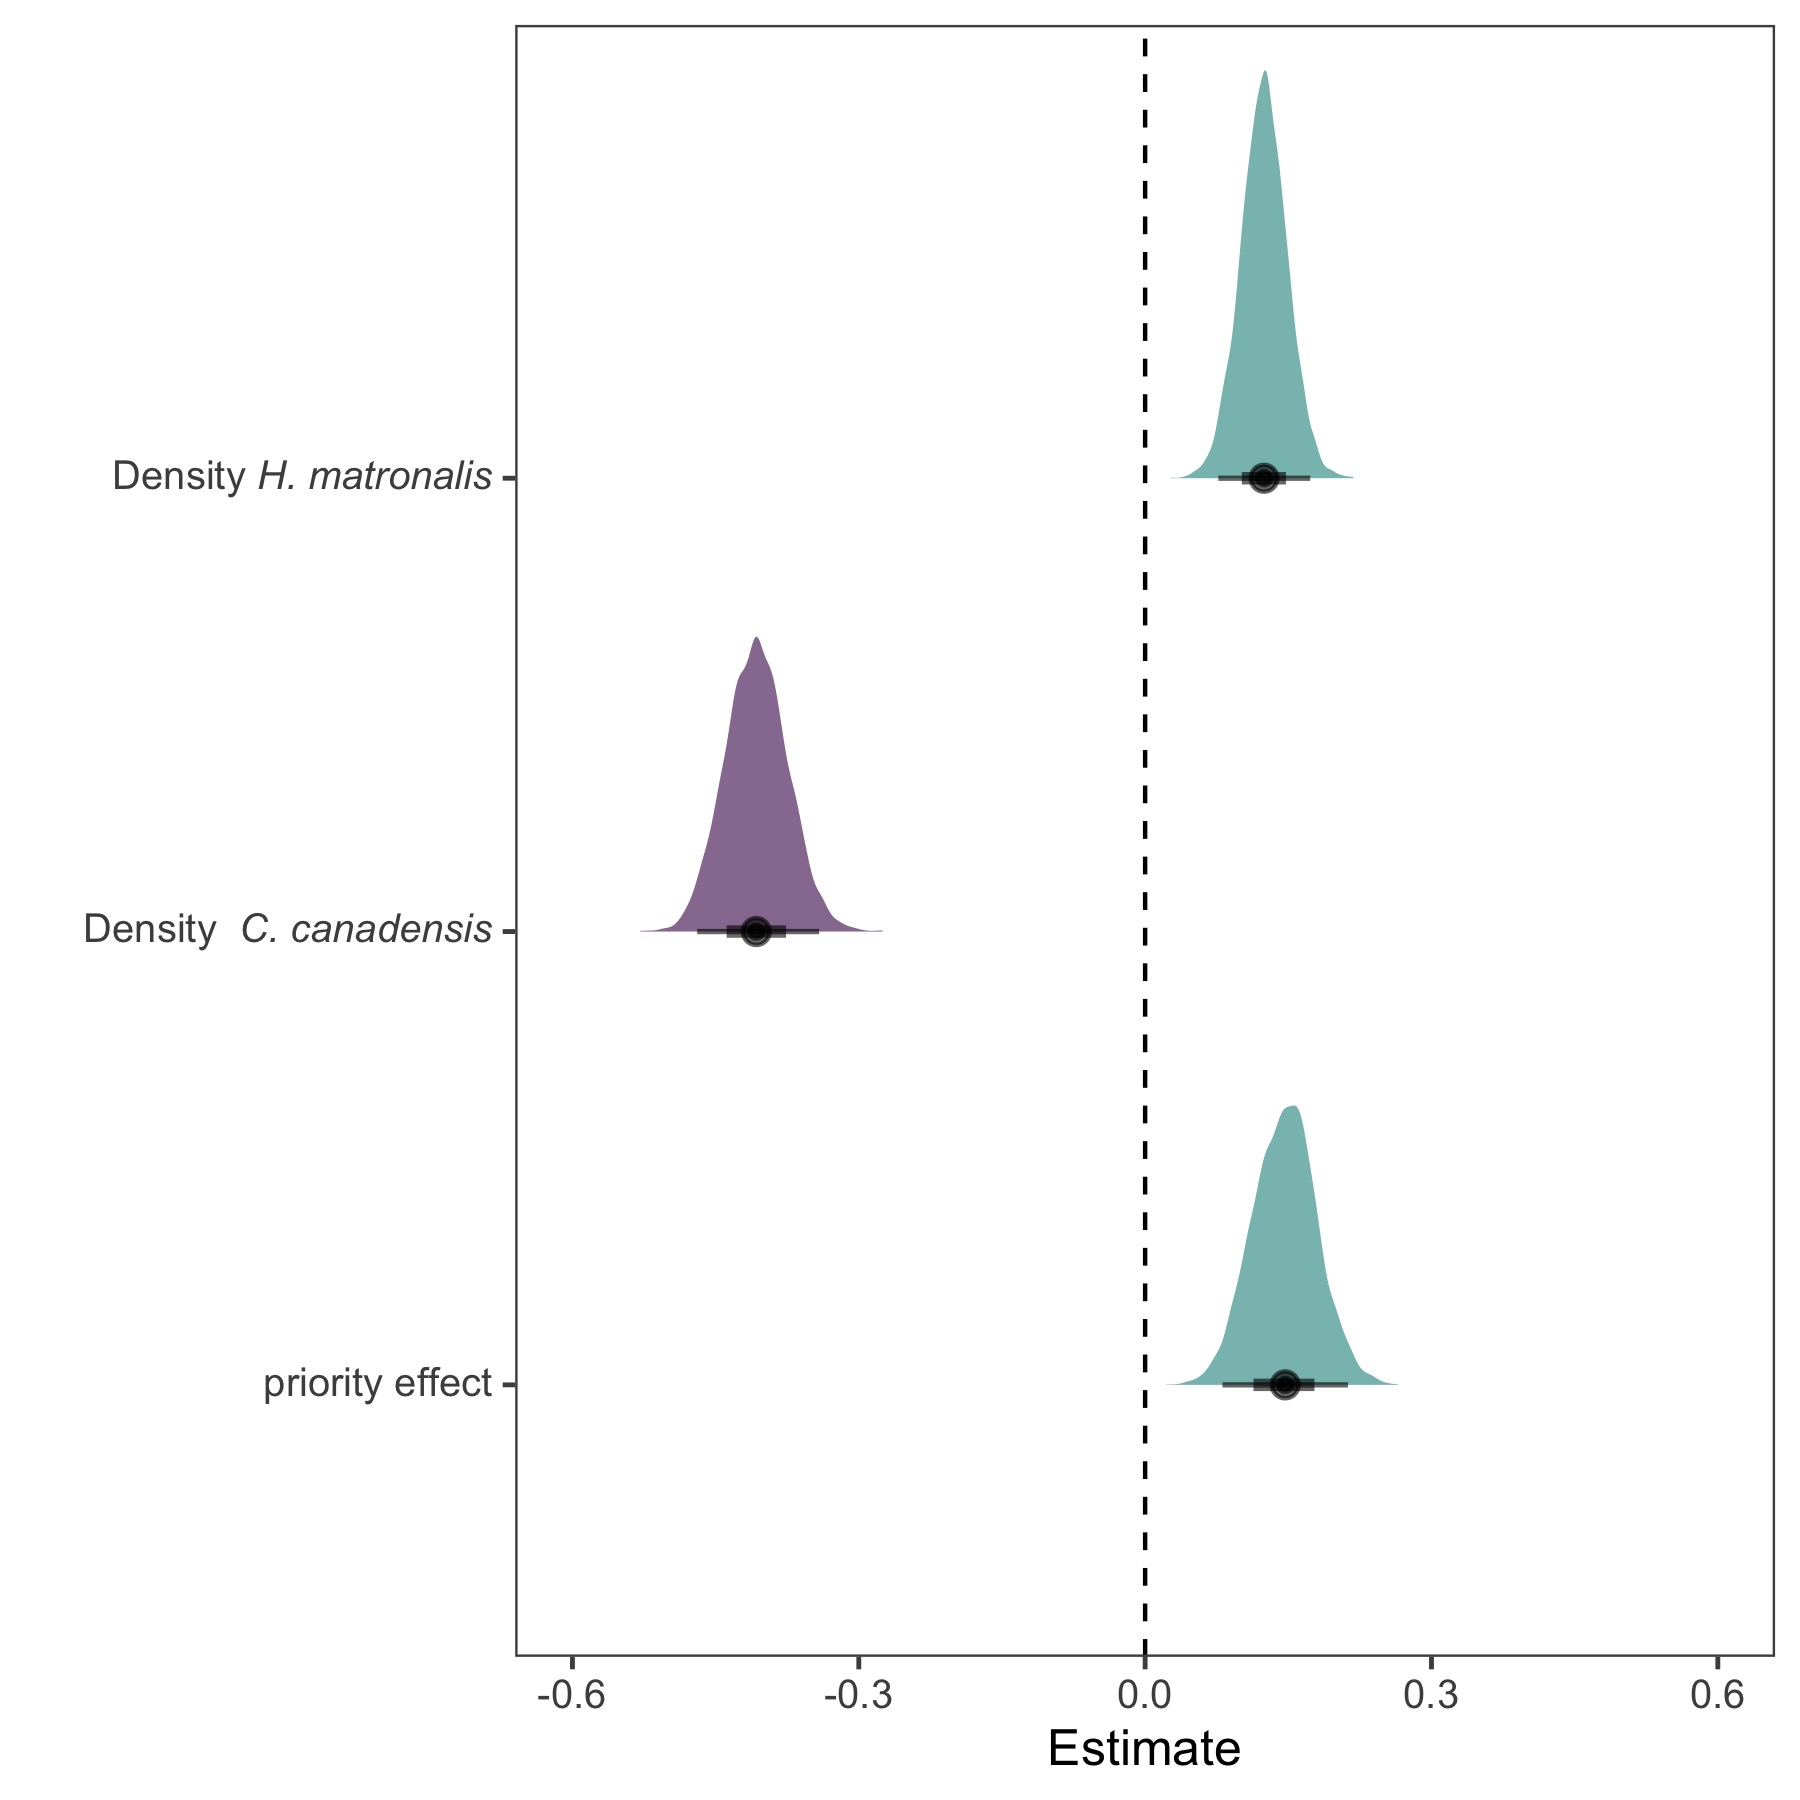
\includegraphics[width=\textwidth]{..//figure/mu_plots.jpeg}
    \caption{Estimated effects of species' abundance (intrinsic competitive ability parameters) and phenological advantage (seasonal priority effects) on the relative growth rate difference between \textit{H. matronalis} and \textit{C. canadensis}. Negative parameter estimates indicate the community biomass composition shifts to favor \textit{C. candensis} while positive estimate towards dominance by \textit{ H. matronalis}. The points indicate the mean estimated effect of each parameter and bars the 90\% uncertainty intervals. The full posterior distribution for each parameter is also depicted as an additional measure of uncertainty.} 
    \label{fig:RGRD}
\end{figure}




\end{document}
